\chapter{Analysis}
This section analyzes how Boolean Networks can be converted from SBML to ERODE format and vice versa. The topic is rather extensive, so the analysis is divided into several subsections. In section 4.1, the definitions and some examples of Boolean and multi-valued networks are given. Section 4.2 shows how these networks are represented in the SBML-qual format. Section 4.3 explains the corresponding network representation in ERODE. Finally, section 4.4 discusses the conversion between the two formats.

%\commentGeorgios{I propose an alternative structure of this section:
%\begin{itemize}
%    \item Boolean and Multivalued Networks
%    \item The structure of SBML-qual models
%    \item Representation of BNs in ERODE
%    \item Conversion between the two formats
%    \begin{itemize}
%        \item qualitative species conversion
%        \item function term conversion
%        \item conversion of logical and relational operators
%    \end{itemize}
%\end{itemize}}

\section{Boolean and Multi-valued networks}

We first give a formal definitions of a Boolean Network as in \cite{argyris2021reducing}. A Boolean network is a pair $(X,F)$ where:
\begin{itemize}
    \item $X=\{x_1, x_2, \ldots ,x_n\}$ is a set of variables, and
    \item $F=\{f_{x_1},f_{x_2}, \ldots, f_{x_n}\}$ is a set of update functions that correspond to each variable of the set $X$.
\end{itemize}

Particularly, $\forall i$ we have that $f_{x_i}:\mathbf{B}^n \to \mathbf{B}$ with $\mathbf{B}=\{0,1\}$.
Figure~\ref{fig:BN} displays a Boolean network on 3 variables i.e. $X=\{x_1,x_2,x_3\}$. We denote with \textbf{x}(t) the vector $(x_1(t),x_2(t),x_3(t))$.

\begin{figure}[h]
    \centering
   			\[
			\begin{array}{rrrcl}
				f_1(\textbf{x}(t))&=&x_1(t+1) &=& \neg x_3(t) \vee x_1(t)\\
				f_2(\textbf{x}(t))&=&x_2(t+1) &=& x_1(t) \vee x_2(t) \vee \neg x_3(t)\\
				f_3(\textbf{x}(t))&=&x_3(t+1) &=& x_2(t) \wedge \neg x_3(t)
			\end{array}
			\]
    \caption{A Boolean network}
    \label{fig:BN}
\end{figure}

A multivalued network is a pair $(X,F)$ where $X$,$F$ are a set of variables and a set of update functions respectively as in Boolean networks. In contrast with Boolean networks, the variables of multivalued networks take values in some discrete domain of the form $\{0,1,2, \ldots, m\}$. Hence, we have that: $\forall i$ $f_{x_i}:\mathbf{D} \to \mathbf{D}_{x_i}$ with $\mathbf{D}=\prod_{i=1}^n \mathbf{D}_{x_i}$. Figure~\ref{fig:MN} displays a multivalued network:
\begin{figure}[H]
    \centering
    $
    \begin{array}{ccl}
        x_1(t+1)&= &
        \begin{cases} 
            2 & (1 \leq x_1(t)) \lor (x_3(t)\geq 1 \land x_1(t)\geq 1) \\
            1 & x_1(t) < 1 \land x_3(t) \geq 1 \\
            0 & otherwise
        \end{cases}
         \\
         \\
         
         x_2(t+1)&= &
        \begin{cases} 
            1 & x_1(t)\geq 1 \\
            0 & otherwise
        \end{cases}
        
        \\
        \\
        
        x_3(t+1)&= & 
        \begin{cases} 
            1 & x_2(t)\geq 1 \\
            0 & otherwise
        \end{cases}
    \end{array}
    $
    \caption{A simple MN}
    \label{fig:MN}
\end{figure}

In this case $\mathbf{D}_{x_1}=\{0,1,2\}$ whereas $\mathbf{D}_{x_2}=\mathbf{D}_{x_3}=\mathbf{B}$. If at least one variable of the set $X$ take values in a domain $\mathbf{D}\neq \mathbf{B}$, the network is considered multivalued.

\section{The structure of SBML-qual models}
All SBML-models are organized in treelike structures, similar to how an abstract syntax tree represents the syntactic structure of a piece of code. The root of the SBML-tree is the \verb+SBML+-element, which specifies the SBML level, the version and the extensions used to represent the model (see Listing 1 below). It also contains the \verb+model+-element, used to represent the model. The contents of the \verb+model+-element varies, depending on the model type and the extensions required to represent it. This project focuses on qualitative models i.e. SBML-files with the -qual extension. SBML-elements that are part of the SBML-qual extension are denoted with the \texttt{qual:}-prefix.

\begin{lstlisting}[language=SBML, caption=Outer structure of an SBML-qual model]
<sbml level="3" version="1"
    xmlns="http://www.sbml.org/sbml/level3/version1/core"
    xmlns:qual="http://www.sbml.org/sbml/level3/version1/..."
    qual:required="true">
        <model>
            <!-- model content-->
        </model>
</sbml>

\end{lstlisting}

The primary structures used to represent SBML-qual models are the \\
\texttt{listOfQualitativeSpecies} and the \texttt{listOfTransitions}. The former defines the model's species, the latter the model's transitions. The species are used to represent the state of the model, whereas the transitions define how the species change state. 

\subsection{Qualitative Species}
 Each species is defined by the following six attributes:
\begin{itemize}
    \item The \textbf{SId} (\texttt{qual:id}) is the unique identifier of the species.
    \item The \textbf{Name} is an optional attribute storing the name of the species.
    \item The \textbf{Compartment} attribute, which indicates in which compartment the given species is located.
    \item The \textbf{Max Level} is another optional attribute indicating the maximum value the species can achieve in any of its states.
    \item The \textbf{Initial Level} an optional attribute that indicates the value of a species in its starting state.
    \item The \textbf{Constant}-attribute is a Boolean value indicating, whether or not the value of the species is constant.
\end{itemize}
\begin{lstlisting}[language=SBML, caption=An example of a qualitative species in SBML-qual]
<qual:qualitativeSpecies qual:id="S_1" qual:name="Species1"
    qual:compartment="comp1"
    qual:maxLevel="1" qual:initialLevel="0"
    qual:constant="false"/>
\end{lstlisting}

\subsection{Transitions}
A transition consists of three defining structures:
\begin{itemize}
    \item A list of \texttt{Output}s containing IDs of the species are affected by the result of the transition.
    \item A list of \texttt{Input}s containing IDs of the species that may affect the outcome of the transition.
    \item A list of \texttt{FunctionTerm}s containing the logical expression that determine the outcome of the transition. All function terms have a \emph{result level} that indicates, what value should be assigned to the species, in case their condition is met. There are two types of function terms in SBML-qual. The regular \texttt{functionTerm} and the \texttt{defaultTerm}. The \texttt{functionTerm} contains a logical expression, written in MathML\*, whereas the \texttt{defaultTerm} is an empty expression that always returns true. It acts as a last resort and assigns a default value to the species if none of the other conditions are met.
    %An XML extension  used to write mathematical expressions
\end{itemize}
In a more legible mathematical notation,  a simple multi-valued transition could look like this:
\begin{align*}
    &\text{Given the Species:} \{S_1,S_2,S_3\} \\
    &S_1 = \begin{cases}
    2 & \text{if}\,S_2 = 1 \land S_3 == 2 \\
    1 & \text{if}\,S_3 \neq 2 \\
    0 & \text{otherwise}
    \end{cases}
\end{align*}
In the example species $S_1$ is the output species, that will be assigned a new value. Species $S_2$ and $S_3$ act as input species, as they are used in the logical expressions, that determine the output value. Finally, the term \emph{otherwise} indicates the default term, which assigns the default value.
Boolean transitions can be expressed in the exact same manner as multi-valued transitions. The only difference between them is, that the Boolean transitions is limited to binary output $\{1,0\}$ (true, false), which means that they always have a single function term in addition to the \emph{otherwise} case. It should also be noted that function terms need to be evaluated with their result levels sorted in descending order, for a transition to be evaluated correctly.
\begin{lstlisting}[language=SBML, caption=The transition example in SBML-qual (simplified)]
<qual:transition>
  <qual:listOfInputs>
    <qual:input qual:qualitativeSpecies="S_2">
    </qual:input>
    <qual:input qual:qualitativeSpecies="S_3">
    </qual:input>
  </qual:listOfInputs>
  <qual:listOfOutputs>
    <qual:output qual:qualitativeSpecies="S_1">
    </qual:output>
  </qual:listOfOutputs>
  <qual:listOfFunctionTerms>
    <qual:defaultTerm qual:resultLevel="0">
    </qual:defaultTerm>
    <qual:functionTerm qual:resultLevel="1">
	  <math xmlns="http://www.w3.org/1998/Math/MathML">
        <!--S_2 == 1 && S_3 == 2 in MathML-->
	  </math>
    </qual:functionTerm>
    <qual:functionTerm qual:resultLevel="2">
      <math xmlns="http://www.w3.org/1998/Math/MathML">
	    <!--S_3 != 2 in MathML-->
	  </math>
    </qual:functionTerm>
  </qual:listOfFunctionTerms>
</qual:transition>
\end{lstlisting}

For a full overview of the SBML and SBML-qual structures it is recommended to take a look at the SBML (\cite{hucka2018systems}) and SBML-qual (\cite{sbmlqual2015}) specifications, which can be found at \href{http://sbml.org/Documents/Specifications}{SBML.org} (\cite{documents/specifications}).


\section{Representation of Boolean networks in ERODE}
SBML and ERODE utilise different data structures to represent species and transitions. In ERODE, the set of values used to define a species only partially overlaps with the set of values used by SBML. However, as both formats are used to represent similar types of models, the overlapping values in the definition sets are the most important ones.

The values of an ERODE species that overlap with those of an SBML species are the \emph{name}, \emph{originalName} and the \emph{initialConcentration}, although their names differ from those used in SBML.
The \emph{name} of an ERODE species and the \emph{id} in SBML both are used to represent the variable name for that species in the model. Also, an ERODE species \emph{originalName} attribute corresponds to the \emph{name} attribute in SBML, since both represent the actual name of the species. The last attribute pair is the \emph{intialConcentration} in ERODE and the \emph{initialLevel} in SBML. Both of these attributes are used to indicate the starting value for the species.

The transition representations differ even more than than the species. Where SBML uses a list to represent its transitions, ERODE uses a HashMap. Additionally, the transitions themselves are also represented differently.
In SBML a the transition data structure contains three items:
\begin{itemize}
    \item a list of \emph{inputs}
    \item a list of \emph{outputs}
    \item a list of \emph{function terms}
\end{itemize}
In ERODE, transitions only have a single output and a single function term, called the update function. These two items form a single entry in the HashMap used by ERODE to store its transitions. In both formats, the output is a reference to the species affected by the result of the transition. In ERODE, this species reference is used as a key, which the function term (update function) is mapped to. The HashMap essentially acts a dictionary that is used by ERODE to look up a species update condition.
The update function structure in ERODE, also differs slightly from the function term used in SBML. In SBML function terms all have a result level indicating the what value will be assigned to the species if their condition is met. However, due to ERODE being limited to the Boolean domain, this is not required. The update function implicitly represents the value $1$ (true) if its condition is met, and $0$ otherwise.

Just like SBML, the species and transition are contained within an outer structure representing the model itself. In ERODE, object instances that implement the \emph{IBooleanNetwork}-interface are used for this.

\section{Conversion between the two formats}
To successfully convert a given network model from one format to the other, it requires that both the \emph{species} and the \emph{transitions} of the model can be converted.
This requires and analysis of which attributes are represented in both representations and which are not.
The common attributes can then be converted by simply transferring their values to the other format. For the other attributes it must be analyzed, whether these attributes are required in the other format, and if so how they can be converted.

\subsection{Converting qualitative species}
As previously mentioned, the species representations of both formats have three matching pairs of data, as shown in the following list. As a note, the SBML attribute is always given first:
\begin{itemize}
    \item The \emph{id} and \emph{name} attributes, which specify the variable name for the species, that is used in the model
    \item The \emph{name} and \emph{originalName} attributes, which represent the actual name of the species
    \item The \emph{initialLevel} and \emph{intitialConcentration} attributes, which specify the initial value of the species
\end{itemize}
For these pairs the only actual conversion that might be required is to change the data type used to represent them, as for example the conversion of the \emph{initialLevel} from SBML to ERODE, as shown in figure \ref{speciesConversion}.

Instead of being represented as in integer like in SBML, the \emph{initialConcentration} in ERODE is represented both as a big decimal type and a string. This particular type conversion however is rather simple, as a big decimal is a special type of integer representation for arbitrary sized integers. 
In addition to this rather complex integer representation, the initial value of a species is also stored in the \emph{initialConcentrationExpr}, a string representation of the initial value. Since the \emph{initial level} of an SBML species is an optional value, the converter can simply use a default value $0$ as the \emph{initial concentration} in case the \emph{initial level} is unset. When converting this attribute back to SBML, a simple type conversion between the two integer types is required, as the possible set of values for the ERODE representation is limited to $\{0,1\}$.

\begin{figure}[H]
    \centering
    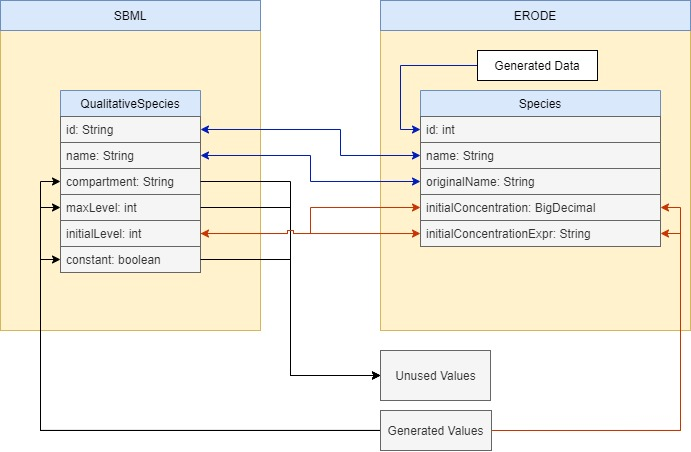
\includegraphics[scale=0.45]{Sections/Images/SpeciesConversionMapping.jpg}
    \caption{Species conversion mapping schema}
    \label{speciesConversion}
\end{figure}

When looking at figure \ref{speciesConversion}, it can also be seen that the species representation used by SBML, which can be found on the left side of the figure, has more attributes than the ERODE representation on the right. This is due to the fact, that ERODE specifies these values implicitly.
Firstly, ERODE does not support declaring species as \emph{constants}. This can only be handled implicitly, for example by not giving those species an update function that would make a value-change possible. Secondly, the \emph{maximum level} is already defined, since ERODE only is capable to represent models within the Boolean domain $\{0,1\}$. Making a successful conversion of a multi-valued network impossible in ERODE's current state. Finally, the \emph{compartment} attribute is a value simply cannot be translated to ERODE format. However, upon speaking with the ERODE's developers about this problem, it was decided that all models can be interpreted as single-compartment models, making this attribute irrelevant. Due to these reasons, these three SBML attributes can be safely discarded during the species conversion to ERODE format. Of course, this also means that these attributes require the generation of default values, when converting back to ERODE format. These default values are:
\begin{itemize}
    \item A default compartment name, that is the same for each species, such as "default"
    \item A maximum level of 1, due to all models being in the Boolean domain.
    \item The \emph{constant} attribute being set to \texttt{false}, as species without transitions cannot \\ change value, even if it is allowed.
\end{itemize}

Finally, the last attribute that needs special treatment during the conversion from SBML to ERODE is ERODE's \emph{id}-attribute. This value is used to give each species a unique identifier within ERODE itself and therefore has no counterpart in SBML. To provide such a value, the converter can simply start a counter during the species conversion, which is incremented each time another species has been converted. Since the counter value changes to a new value after each iteration, the counter value can be used as an \emph{id} for the ERODE species.



%As it can be seen in the conversion schema above, not all attributes of an SBML-species are required in ERODE, which means that they have to be discarded during conversion. Discarding data during conversions is always dangerous, as it can severely impact the quality of the conversion. Seeing that the SBML-attributes \emph{compartment}, \emph{maxLevel} and \emph{constant} are discarded, means that there are a few limitations to which kinds of networks can be converted to ERODE format correctly. \comg{The last sentence needs to be rewritten better. Break it into two sentences.}.\comg{Particularly, the limitations identified during our analysis are summarized in the following:}

%\begin{itemize}
%    \item All species in the network must be in the same compartment, therefore multi-compartment networks cannot be represented correctly. 
%    \item A maximum value of a species cannot be specified, which means that multi-valued networks cannot be represented in ERODE. 
%    
%    \item ERODE species cannot be constant. This means that the species update function (transition) needs to ensure that its value never changes, in order to represent the species correctly. 
    
%\end{itemize}
%Another problem that can arise, when converting an qualitative Species to ERODE format, is that ERODE requires an \emph{initialConcentration} \comg{In ERODE the initial value is also an optional attribute!}. In SBML this corresponds to the \emph{initialLevel}-attribute, which is an optional attribute. This means, that a default concentration needs to be generated by the converter, in case the \emph{initialLevel} is unset in SBML.

%When converting ERODE data to SBML format, it is also evident that ERODE cannot supply all data required by SBML. Luckily, this is not a problem, since most of the missing data are given by ERODE's restrictions to its supported models or are optional data in SBML. For required fields in SBML, that do not exist in ERODE, it is possible to assign default values, as they are defined by ERODE's limitations. The \texttt{constant}-field can be assigned the value \texttt{false}, since species in ERODE do not have a \textit{constant}-property. Also, all ERODE models are represented in a single compartment, which means that every species can be assigned to the same compartment, when converting to SBML. The last missing property, the maximum level is an optional parameter in SBML, but can be assigned a default value as well. Since ERODE currently only support BNs, the values of each species are restricted to the Boolean domain ${0,1}$, which means that the maximum level could be set to $1$ by default, but this is not required for a successful conversion. 

\subsection{Transition conversion}
Converting a transition from SBML to ERODE is much simpler than the conversion of a species, since ERODE requires a lot less data from the SBML representation. The drawback of this is that the converter needs to generate a lot more data, when converting back to SBML. This is due to SBML being an extensive format, that can be used to represent a large variety of model types.

as shown in figure \ref{fig:transitionConversion}, the conversion of an SBML transition to ERODE format requires a reference to the updated species and an update condition to be supplied. In SBML these attributes are contained in the \emph{outputs} and \emph{function terms} of a transition. The \emph{outputs} are a list containing references to each species updated by the given SBML transition. The \emph{function terms} are a list of items representing the condition, when to apply which result level. Since ERODE only supports models from the Boolean domain, only the function term for the result level $1$ (true) is required, since ERODE handles the \emph{otherwise}-case implicitly. 

Before a \emph{function term} can be used to represent a ERODE transition, the logical expression it contains must be converted to ERODE format. This is required, because both formats use different implementations to represent abstract syntax trees (ASTs), a data structure used to express mathematical expressions unambiguously.
Once the expression has been converted, the resulting expression (the update function) is used to create an entry in the LinkedHashMap, for each species referenced in the list of outputs. This creates a dictionary in ERODE, that can be used to look up, which species require which condition to be true, to change to the \emph{true}-state.

\begin{figure}[H]
    \centering
    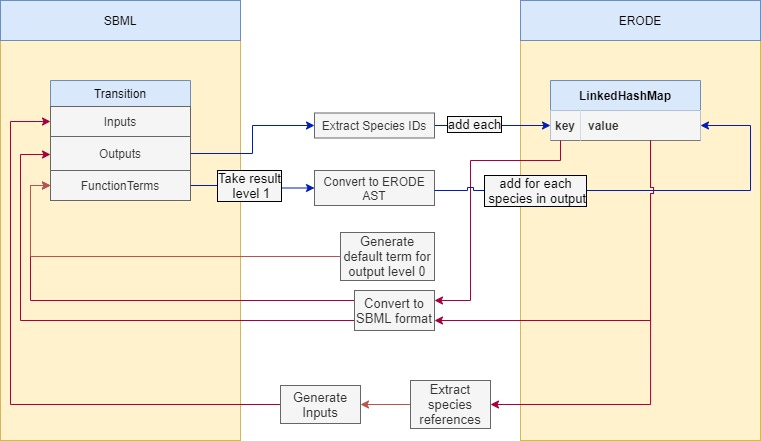
\includegraphics[scale=0.45]{Sections/Images/TransitionConversion.jpg}
    \caption{Converting transitions between SBML and ERODE}
    \label{fig:transitionConversion}
\end{figure}

When converting to SBML format, lists for the \emph{inputs}, \emph{outputs} and \emph{function terms} must be created for the generation of an SBML transition. The \emph{inputs} store information about the species referenced in the function terms of the transition. To generate an input-instance three pieces of information are required:
\begin{itemize}
    \item A string \emph{id}, to specify the unique identifier for the input
    \item The name of the variable used to reference a given species in the function term, stored in the \emph{qualitativeSpecies}-parameter
    \item A \emph{transitionEffect} that specifies how the input is affected by during the transition. This can always be set to \texttt{none}, since ERODE does not support transition effects.
\end{itemize}
To generate these \emph{inputs}, the converter needs to analyze the update function mapped to a species and find each variable used in the function expression. For each new variable found, a new input needs to be generated, duplicates can be skipped. This step is shown at the bottom of figure \ref{fig:transitionConversion}.

The list of \emph{outputs} stores similar information, but about the species that are modified by the transition. Just like \emph{inputs}, each \emph{output} requires an \emph{id}, a reference to a \emph{qualitativeSpecies} and the specification of a \emph{transitionEffect}. The only difference is, that the \emph{transitionEffect} needs to be set to \texttt{assignmentLevel}, since the values of the \emph{output}-species are overwritten by the transition. The only piece of information that is required from ERODE to generate an \emph{output}-instance, is the variable used for the species. The species references, which are used as keys in the \emph{LinkedHashMap}, can be used for the \emph{output}-generation.

Finally, to generate the list of function terms required by each transition instance, the update functions contained in the ERODE's hash map, can be used to genreate \emph{function terms} for the result level $1$ (true). This simply requires a format conversion of the AST represented in the update function. However, for the list of \emph{function terms} to be complete, another function term needs to provided. This is necessary, because SBML requires all possible outcomes of a transition to be defined by a function term. The converter must therefore generate a \emph{default term}, a special condtion-free function term, with a result level of $0$ (false). This \emph{default term} represents the \emph{otherwise}-case in the formal notation of a Boolean or multi-valued network.
Once all three lists have been generated, the converter can generate the converted SBML-transition.

Regarding the conversion between SBML and ERODE, all requirements for the conversion of Boolean networks have now been covered. For a deeper understanding of SBML (\cite{hucka2018systems}) and SBML-qual (\cite{sbmlqual2015}), it is therefore  recommended to take a look at their specifications.  and SBML-qual  specifications, which can be found at  \href{http://sbml.org/Documents/Specifications}{SBML.org} (\cite{documents/specifications}).

%Compared to the conversion of species, the conversion of transitions should be relatively easy, as both formats represent the same mathematical structure, a piece-wise logical function. The problem  is the fact that SBML is a format designed to support a much wider spectrum of network transitions than ERODE. This means, that there once again are limitations to, which SBML-transitions can be represented by ERODE accurately.
%The unsupported SBML properties in this case are, the \texttt{transitionEffect}'s for both transition \texttt{input}s and \texttt{output}s. Both transition effects define how the input or output are affected by the transition.

%In ERODE's network representations transitions do not affect transition \emph{input}s and assign their result to the transition \emph{output}. This is also supported by SBML by setting the transition effect of each input to \emph{none} and to \emph{assignmentLevel} for outputs. As the tranisition effect names might suggest, \emph{none} means that there is no effect on the inputs, whereas the \emph{assignmentLevel} transition effect will assign a new value to the output.
%Converting SBML-transitions can become problematic once the \emph{transition effects} differ from these mentioned cases. Instead of \emph{none}, input transition effects can be set to \emph{consumption}, which means that the \emph{input species} would be reduced during the transition, causing it to change value.  For outputs, the \emph{transition effect} could also be set to \emph{production}, causing the transition to add its result level to the output, instead of replacing it.
%Luckily, both the \emph{consumption} and the \emph{production} transition effects are typically be applied to \emph{multi-valued networks}, which are not supported by ERODE.
%\comg{The \emph{consumption} and \emph{production}, as input and output transition effects, refer to the Petri Net formalism wherein transitions consume tokes from input places.}
%If they were to be applied to a Boolean network in SBML, such a BN could not be represented by ERODE accurately, as the required operations to realize these transition effects are not supported.

%In order to actually convert a transition from SBML to ERODE format, given a correct conversion is possible, it simply requires the extraction of transition outputs and the function term with the result level of $1$ (true). Since all inputs already are referenced in the functions term and the input properties are reflected in it, the list of inputs is not required for the conversion of Boolean networks.
%Since each output references the species to be changed by its id, the only actual conversion step required, is the translation of the logical expression contained in the function term.

%This is a fairly simple operation, as the logical expression is given in the form of an abstract syntax tree (AST), that indicates the structure of the expression. In ERODE the same approach is utilized, just with different representations for the node in the AST. By translating each node in SBML's AST to a corresponding structure in ERODE, it is therefore possible to replicate the same AST in ERODE format, resulting in a converted logical expression.

%The final step is then to add the converted transition by adding it to the \emph{LinkedHashMap} storing all transitions (update functions) of the BN, by inserting the species ID, given by the transition output, as a key and adding the converted logical expression as the value mapped to the key.

%\begin{figure}[H]
%    \centering
%    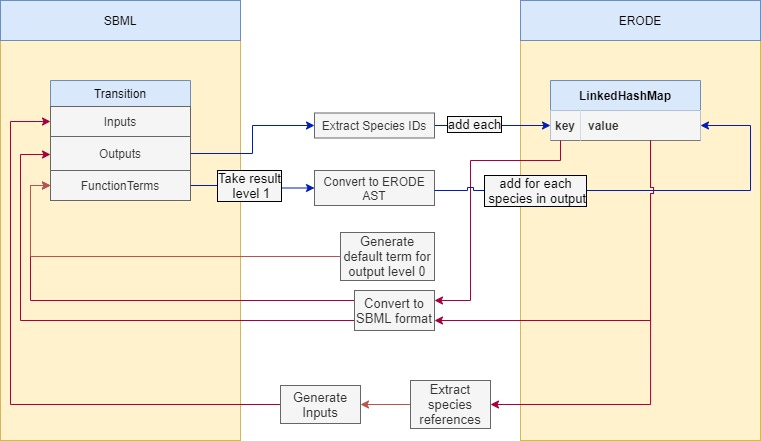
\includegraphics[scale=0.45]{Sections/Images/TransitionConversion.jpg}
%    \caption{Converting transitions between SBML and ERODE}
%    \label{fig:transitionConversion}
%\end{figure}

%As ERODE's transition format does not store any information about transition inputs outside of its function term, converting ERODE transitions back to SBML requires the generation of inputs, for the SBML transition.\comg{I think I can understand what you say here, but please be ore precise: for example. what is the ERODE's transition format.}
%This can be achieved by analysing the logical expression, collecting every new species reference it contains to species in the network. Once all inputs, outputs, and function terms have been generated from the ERODE data and stored in lists, it is then possible to generate the SBML transition from these lists.
%\comg{We can achieve the reverse conversion by following the steps:
%\begin{itemize}
%    \item We obtain from every logical expression (i.e. update function) the key (i.e. the output species).
%    \item We store them into lists.
%    \item Based on these lists, we generate the SBML transitions.
%\end{itemize}}

\subsection{Conversion of logical and relational operators}
Although the principle, how to convert a logical expression from SBML to ERODE format, is quite simple, the operator interfaces of both formats have not been taken into account so far. To be able to convert all valid logical expressions, it requires that all operators in one format, can be expressed using the available operators of the other format. To verify that this is indeed possible, an overview of both operator interfaces is required. The overview is shown in the following table:
\begin{table}[H]
    \centering
    \begin{tabular}{|c|c|c|}
    \hline
    Operator & SBML compatible & ERODE compatible    \\
    \hline
    AND $\land$ & \gcheck & \gcheck \\
    OR $\lor$ & \gcheck & \gcheck \\
    XOR $\oplus$ & \gcheck & \xcheck \\
    NOT $\neg$ & \gcheck & \gcheck \\
    IMPLIES $\rightarrow$ & \gcheck & \gcheck \\
    XNOR (binary equality) $\leftrightarrow$ & (\xcheck) & (\xcheck) \\
    EQUALS $=$ & \gcheck & \xcheck \\
    NOT EQUALS $\neq$ & \gcheck & \xcheck
    
\end{tabular}
    \caption{Operators usable in logical expressions for BNs and their support}
    \label{tab:operators}
\end{table}
When looking at table \ref{tab:operators} above, it can be seen the \texttt{XOR}, \texttt{XNOR}, \texttt{EQUALS} and \texttt{NOT EQUALS} operations are not supported by ERODE. This means that these missing operators need to be expressed using a combination of the existing operator set.

\subsection{The XNOR- and XOR-operation}
The \texttt{XNOR} operator does not exist in either formats, yet it could be used in logical expressions. SBML does not support the \texttt{XNOR} operator because it corresponds to a negated \texttt{XOR} ($\neg{\oplus}$) operation. Since both operators required to expression the \emph{XNOR}-operation already are supported by SBML, there is no need for a separate operator. ERODE, on the other hand, does not support the \texttt{XOR} operation. This means, it has to be constructed using the available operators.

Given two variables $P$ and $Q$, the \texttt{XOR}-operation is defined to be true, if either $P$ or $Q$ are true, but not both. In propositional logic, this condition can be expressed as: 
\[
(P \lor Q) \land \neg{(P \land Q)}
\]
\begin{table}[H]
    \centering
    \begin{tabular}{|c|c|c|c|c|}
    \hline   
    $P$ & $Q$ & $(P \oplus Q)$ & $(P \lor Q) \land \neg{(P \land Q)}$ & $P \oplus Q = (P \lor Q) \land \neg{(P \land Q)}$  \\
    \hline
    T & T & F & F & T \\
    T & F & T & T & T \\
    F & T & T & T & T \\
    F & F & F & F & T \\
    \end{tabular}
    \caption{Truth table verification that \texttt{XOR} is equivalent to $(P \lor Q) \land \neg{(P \land Q)}$}
    \label{tab:verified_xor}
\end{table}
As it can be seen in the truth table \ref{tab:verified_xor} above, the two logical expressions are equivalent, which means that the \texttt{XOR}-operation can be translated to ERODE format using its supported operators.

\subsection{Equality and inequality operators}

Just like the \texttt{XNOR}-operation, the inequality operation can be constructed by negating the equality operator. However, neither equality operator is currently supported by ERODE. Fortunately, the equality can be expressed differently, depending on the domain it is used in.

In the Boolean domain, the \texttt{XNOR}-operation also represents binary equality: it is true if both sides are true, or both sides are false. Since \texttt{XOR} is the opposite of \texttt{XNOR}, the \texttt{XOR}-operator must be equivalent to the inequality-operator. So the big question is, why not just translate these operators to their corresponding logical equivalents?

To answer this question, it is necessary to take ERODE's current state into account. The program is under development and it is intended to implement support for multi-valued networks. In other words, ERODE will eventually support models outside the Boolean domain. Since this converter should be able to convert SBML-qual models into ERODE format, it would be wise to design the converter such that the changes required to adapt to new version of ERODE are minimal.

Since ERODE is restricted to the Boolean domain and these relational operators need to be supported; A good midway would be to implement them in the Boolean domain, while making them as independent from the other operators as possible. This means finding an expression, that has a minimal overlap with the \texttt{XOR}- and \texttt{XNOR}-operators.

This can be realized using the \texttt{implies}-operator. This is due to the fact, that logical equality also corresponds to the \emph{if and only if}-conditional ($\leftrightarrow$) in propositional logic. The conditional can be expressed using the \texttt{implies}-operator, thereby making it highly independent from the other operators.
\[
    A \leftrightarrow B = (A \rightarrow B) \land (B \rightarrow A)
\]
To prove that $(A \rightarrow B) \land (B \rightarrow A)$ only is true, when $A$ and $B$ are equal, consider the possible outcomes of an implication:
\begin{table}[H]
    \centering
    \begin{tabular}{|c|c|c|}
        \hline
         A & B & $A \rightarrow B$  \\
         \hline
         T & T & T \\
         T & F & F \\
         F & T & T \\
         F & F & T \\
         \hline
    \end{tabular}
    \caption{Outcomes of an implication given $A$ and $B$}
    \label{tab:implies}
\end{table}
As it can be seen in table \ref{tab:implies}, the only way for an implication to be false, is when the first argument is true and the latter false. This is also, why $(A \rightarrow B) \land (B \rightarrow A)$ cannot be true, when the two arguments are different, as shown below.
\begin{align}
    &A \rightarrow B &= F \\
    &B \rightarrow A &= T \\
    \hline
    &(A \rightarrow B) \land (B \rightarrow A) &= T \land F & &\text{from (4.1) and (4.2)} \\
    &T \land F &= F& &\text{from (4.3)}\\
    \hline
    &(A \rightarrow B) \land (B \rightarrow A) &= F& &\text{from (4.4)}
\end{align}

Since it has been shown, that equality can be expressed as $(A \rightarrow B) \land (B \rightarrow A)$ in the Boolean domain, it is also evident that inequality would be its negation, This means, that the required relational operators can be converted from SBML to ERODE without having great similarity to the \texttt{XOR}- and \texttt{XNOR}-operators.

It has now been shown that all supported by SBML can be expressed using a combination of ERODE's operators. Unfortunately, these expression conversions cause a significant loss in readability, due to their lengthiness. The expression length problem is especially severe, when it comes to the \emph{equality} and \emph{inequality} operations, since these are used very frequently in the SBML format. Their high usage is due to the fact that many networks are represented using a multi-valued notation (integer based notation) restricting the model to use comparison operations, for operations on variables and constants. This also extends to networks that are within the Boolean domain, as all Boolean models are a subset of all the possible multi-valued models.

To solve the problem of lengthy and unreadable expressions, it would require to update ERODE and extend its operator interface. With this update, the original expression could be maintained and the conversion would have no impact on its readability. Once the developers were presented with this problem, they did eventually decide to extend the operator interface to support the same operator set as SBML. 